\documentclass[../Main.tex]{subfiles}

\begin{document}
\section{Faraday's Law of Induction}
We are interested in the third Maxwell equation:
\begin{equation*}
    \nabla \times \vec{E} = -\frac{\partial B}{\partial t} \tag{\ref{eqnMEC}}.
\end{equation*}
This implies that a time-dependent magnetic field must be accompanied by an electric field. This can induce a current to flow in a conductor, a process known as electromagnetic induction.
\subsection{Faraday's Law for a Static Circuit}
Consider a closed curve $C$ that is the boundary of a time-independent open surface $C$. We integrate \eqnref{eqnMEC} over $S$ and use Stokes's Theorem:
\begin{equation*}
    \int_C \vec{E} \cdot \vec{dx} = -\int_S \frac{\partial \vec{B}}{\partial t} \cdot \vec{dS} = - \frac{d}{dt} \int_S \vec{B} \cdot \vec{dS}
\end{equation*}
This is \underline{Faraday's law of Induction}. We also write it:
\begin{equation*}
    \emf = \frac{d\flux}{dt}
\end{equation*}
Here
\begin{equation*}
    \emf = \int_C \vec{E} \cdot \vec{dx}
\end{equation*}
is the \underline{electromotive force} (emf) around $C$ and
\begin{equation*}
    \flux = \int_S \vec{B} \cdot \vec{dS}
\end{equation*}
is the \underline{magnetic flux} through $S$.

Since $\nabla \cdot \vec{B} = 0$, the flux $\flux$ is the same for any surface $S$ such that $\partial S = C$, and so $\flux$ can be understood to be a property of $C$. In this case, we say $\flux$ is the flux through $C$.

Using $\vec{B} = \nabla \times \vec{A}$ and Stokes's Theorem, we can write
\begin{equation*}
    \flux = \int_C \vec{A} \cdot \vec{dx}
\end{equation*}
which is invariant under a gauge transformation $\tilde{\vec{A}} = \vec{A} + \nabla \chi$. This makes the fact that $\flux$ depends on $C$ and not $S$ clear.

The emf is not actually a force. It is the line integral of the Lorentz force on a particle of unit charge confined to $C$:
\begin{equation*}
    \emf = \frac1q \int_C \vec{F} \cdot \vec{dx} = \int_C (\vec{E} + \dvec{x} \times \vec{B}) \cdot \vec{dx} = \int_C \vec{E} \cdot \vec{dx}
\end{equation*}
since $\dvec{x}$ is tangent to $C$ for a particle confined to $C$ (and assuming $C$ is time-independent).

We will see later that if $C$ coincides with a thin wire of resistance $R$, then the current induced in the wire is $I = \emf / R$.

There are several ways in which the magnetic flux through $C$ could change in time:
\begin{itemize}
    \item a magnet is moved near $C$;
    \item a current-carrying circuit is moved near $C$;
    \item the current flowing in a nearby circuit is changed.
\end{itemize}
All these will induce an emf around $C$ and cause a current to flow.
\subsection{Faraday's Law for a Moving Circuit}
Noe let $C(t)$ be a \underline{time-dependent} closed curve that is the boundary of an open surface $C(t)$. Then we want to understand how the magnetic flux,
\begin{equation*}
    \flux(t) = \int_{S(t)} \vec{B}(\vec{x}, t) \cdot \vec{dS}
\end{equation*}
changes in time.

Consider a small time interval $\delta t$ and expand the difference in $\flux$ to first order.
\begin{align}
    \flux(t + \delta t) &- \flux(t) = \int_{S(t + \delta t)} \vec{B}(\vec{x}, t + \delta t) \cdot \vec{dS} - \int_S \vec{B}(\vec{x}, t) \cdot \vec{dS} \nonumber \\
    &= \int_{S(t + \delta t)} \left(\vec{B}(\vec{x}, t) + \frac{\partial \vec{B}}{\partial t} \delta t + O(\delta t^2)\right) \cdot \vec{dS}\nonumber\\
    &\qquad- \int_{S(t)} \vec{B}(\vec{x}, t) \cdot \vec{dS} \label{eqnFluxDifference} \\
    &= \int_{S(t + \delta t) \backslash S(t)} \vec{B}(\vec{x}, t) \cdot \vec{dS} + \int_{S(t)} \frac{\partial \vec{B}}{\partial t} \cdot \vec{dS}~\delta t _ O(\delta t^2) \nonumber
\end{align}
To resolve the first term, let $\delta V$ be the volume swept out by $S(t)$ in the time interval $\delta t$. Its boundary is the closed surface $S(t + \delta t) \backslash S(t) \cup \Sigma$ where $\Sigma$ is the surface swept out by $C(t)$ in the $\delta t$. See figure~\ref{figTimeDepSurface}.

\begin{figure}
    \centering
    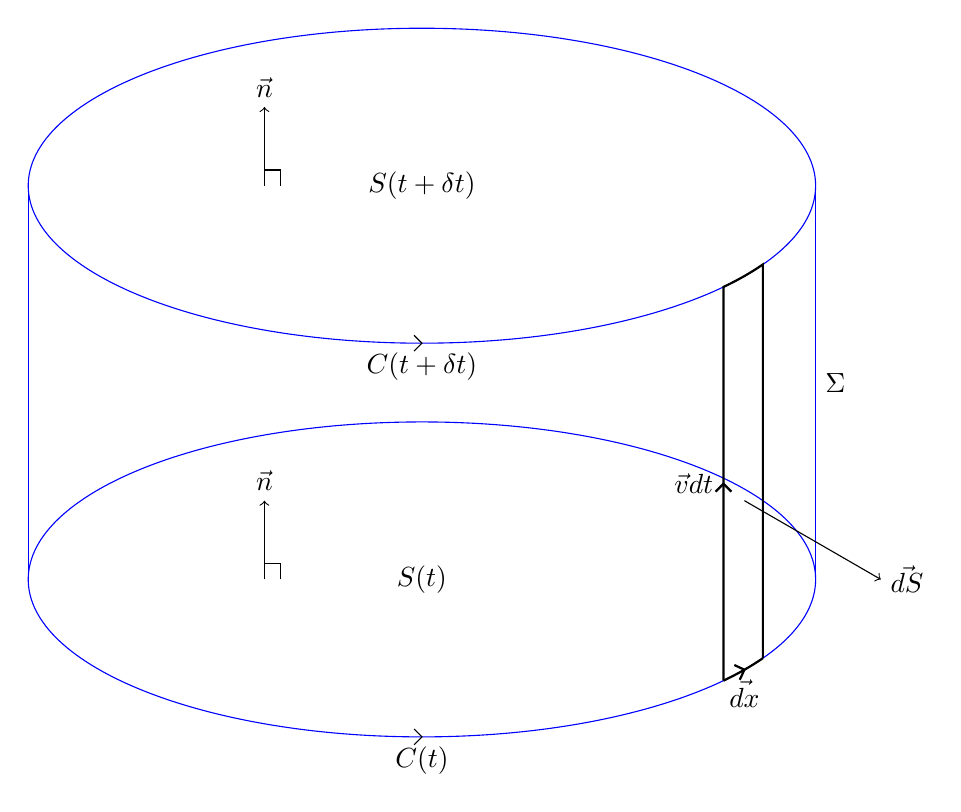
\begin{tikzpicture}
        \tikzset{linearrow/.pic={
        \draw (-0.1, -0.1) -- (0, 0) -- (0.1, -0.1);
        }}
        \draw[blue] (0, 0) ellipse[x radius=5, y radius=2];
        \draw[blue] (0, 5) ellipse[x radius=5, y radius=2];
        \draw[blue] (-5, 0) -- (-5, 5);
        \draw[blue] (5, 0) -- (5, 5);
        
        \draw (0, -2) pic[rotate=-90] {linearrow}
            node[anchor=north] {$C(t)$};
        \draw (0, 3) pic[rotate=-90] {linearrow}
            node[anchor=north] {$C(t + \delta t)$};

        \node at (0, 0) {$S(t)$};
        \node at (0, 5) {$S(t + \delta t)$};

        \foreach \y in {0, 5} {
            \draw[->] (-2, \y) -- ++(0, 1) node[anchor=south] {$\vec{n}$};
            \draw (-1.8, \y) -- ++(0, 0.2) -- ++(-0.2, 0);
        }

        \node[anchor=west] at (5, 2.5) {$\Sigma$};

        \pgfmathsetmacro{\arcx}{5 * cos(-40)}
        \pgfmathsetmacro{\arcxcentre}{5 * cos(-35)}
        \pgfmathsetmacro{\arcy}{2 * sin(-40)}
        \pgfmathsetmacro{\toparcy}{\arcy + 5}

        \draw[thick] (\arcx, \arcy) arc[start angle=-40, end angle=-30, x radius=5, y radius=2]
            pic[pos=0.5, rotate=-70] {linearrow}
            node[pos=0.5, anchor=north] {$\vec{dx}$};

        \draw[thick] (\arcx, \arcy) -- (\arcx, \toparcy)
        pic[pos=0.5] {linearrow}
        node[pos=0.5, anchor=east] {$\vec{v} dt$}
        arc[start angle=-40, end angle=-30, x radius=5, y radius=2] -- ++(0, -5);

        \draw[->] (\arcxcentre, 1) -- ++(-30:2)
            node[anchor=west] {$\vec{dS}$};
        
    \end{tikzpicture}
    \caption{Diagram of a time-dependent surface}
    \label{figTimeDepSurface}
\end{figure}

Then by \eqnref{eqnMBD},
\begin{align*}
    0 &= \int_{\delta V} \nabla \cdot \vec{B} dV \\
    &= \int_{S(t + \delta t) \backslash S(t)} \vec{B} \cdot \vec{dS} + \int_\Sigma \vec{B} \cdot \vec{dS} \\
\end{align*}
to evaluate the last term, parameterise $C$ as $\vec{x} = \vec{x}(\lambda, t)$ where $\lambda$ is a parameter around $C$. An element of $C$ is:
\begin{equation*}
    \vec{dx} = \frac{\partial \vec{x}}{\partial \lambda} d\lambda
\end{equation*}
and has velocity $\vec{v} = \frac{\partial \vec{x}}{\partial t}$.

In time $\delta t$ it sweeps out the vector area element:
\begin{equation*}
    \vec{dS} = \vec{dx} \times (\vec{v} \delta t)
\end{equation*}
and by considering the diagram, this points out of $\delta V$, are required. Therefore:
\begin{equation*}
    \int_\Sigma \vec{B} \cdot \vec{dS} = \int_C \vec{B} \cdot \left(\vec{dx} \times \vec{v}\right) \delta t + O(\delta t^2).
\end{equation*}
Returning to \eqnref{eqnFluxDifference}:
\begin{align*}
    \flux(t + \delta t) - \flux(t) &= - \int_C (\vec{v} \times \vec{B}) \cdot \vec{dx}~\delta t + \int_S \frac{\partial \vec{B}}{\partial t} \cdot \vec{dS}~\delta t + O(\delta t^2) \\
    \frac{d\flux}{dt} &= -\int_C (\vec{v} \times \vec{B}) \cdot \vec{dx} + \int_S \frac{\partial \vec{B}}{\partial t} \cdot \vec{dS} \\
    &= -\int_C (\vec{v} \times \vec{B}) \cdot \vec{dx} - \int_S (\nabla \times \vec{E}) \cdot \vec{dS} \\
    &= -\int_C (\vec{E} + \vec{v} \times \vec{B}) \cdot \vec{dx}
\end{align*}
Therefore we recover Faraday's Law, $\emf = -\frac{d\flux}{dt}$ with the redefined emf:
\begin{equation*}
    \emf = \int_C (\vec{E} + \vec{v} \times \vec{B}) \cdot \vec{dx}
\end{equation*}
This is again given by the line integral around $C$ of the Lorentz force on a particle of unit charge confined to $C$ (for which the perpendicular components of $\dvec{x}$ must agree with those of the curve velocity $\vec{v}$).
\begin{remark}
    Since we can choose any parameterisation $\lambda$, the curve velocity could have any number of tangential components (based on how the parameterisation moves around $C$), and so this is the strongest condition we could impose on $\dvec{x}$.
\end{remark}
\subsection{Lenz's Law}
Lenz's law states that the direction of the induced current is always such as to produce a magnetic field that opposes the change in flux that caused the emf.
\begin{example}
    Consider a circular wire in the $xy$-plane. If $B_z$ inside the loop increases in time then:
    \begin{equation*}
        \emf = -\frac{d\flux}{dt} < 0
    \end{equation*}
    which will induce a clockwise current around the loop ($I < 0$), which will generate a magnetic field $B_z < 0$ inside the loop. This avoid an unstable situation of positive feedback.
\end{example}
\section{Inductance and Magnetic Energy}
\subsection{Inductance}
\begin{definition}{Inductance}
    If a current $I$ around a circuit $C$ generates a magnetic field with flux $\flux$, then the \underline{inductance} of the circuit is defined by:
    \begin{equation*}
        L = \frac{\flux}{I}
    \end{equation*}
    and depends only on the geometry of the circuit (since $\flux$ is proportional to $I$).
\end{definition}
\begin{example}[Inductance of an Ideal Solenoid]
    Consider an ideal solenoid with cross-sectional area $A$ and $N$ turns per unit length. The magnetic field inside the solenoid is uniform:
    \begin{equation*}
        \vec{B} = \mu_0 N I \vec{e_z}.
    \end{equation*}
    Then the magnetic flux passing through this solenoid is $BA$ per turn, so the inductance per unit length is:
    \begin{equation*}
        l = \mu_0 N^2 A
    \end{equation*}
\end{example}
\begin{example}[Mutual inductance between two wires]
    Consider a thin wire $C_i$. Let the current around another thin wire $C_j$ be $I_j$. Then the flux through $C_i$ is:
    \begin{equation*}
        \flux_{ij} = L_{ij} I_j
    \end{equation*}
    where
    \begin{equation*}
        L_{ij} = \frac{\mu_0}{4\pi} \int_{C_i} \int_{C_j} \frac{\vec{dx_i} \cdot \vec{dx_j}}{|\vec{x_i} - \vec{x_j}|}
    \end{equation*}
    %TODO: Derive this with the magnetic vector potential.
\end{example}
\subsection{Changes in Current and Electromagnetic Energy}
When the current $I$ around a circuit $C$ is varied, an emf is induced:
\begin{equation*}
    \emf = -\frac{d\flux}{dt} = -L \frac{dI}{dt}
\end{equation*}
In a small time interval $\delta t$, a charge $\delta Q = I \delta t$ flows around the circuit and the work done on it by the Lorentz force is:
\begin{equation*}
    \delta W = \emf~\delta Q = -LI \frac{dI}{dt} \delta t
\end{equation*}
Then the rate at which work is done by the current on the electrogmagnetic field is:
\begin{equation*}
    -\frac{dW}{dt} = LI \frac{dI}{dt} = \frac{d}{dt} \left(\frac12 LI^2\right).
\end{equation*}
Consider reaching a magnetostatic state by building up the current from 0. Then the energy stored in this configuration is:
\begin{equation*}
    \int_0^t \frac{d}{dt} \left(\frac12 LI^2\right) dt = \frac12 LI^2
\end{equation*}
As with capacitance, we can also write:
\begin{align*}
    U &= \frac12 LI^2 \\
    &= \frac12 I \flux \\
    &= \frac12 I \int_C \vec{A} \cdot \vec{dx} \\
    &= \frac12 \int_{\R^3} \vec{J} \cdot \vec{A} dV
\end{align*}
which we can compare to the energy stored in an electric field:
\begin{equation*}
    U = \frac12 \int_{\R^3} \rho \Phi dV.
\end{equation*}
In electrostatics, we then converted this into an integral involving $|\vec{E}|^2$. In the case of magnetostatics, we apply \eqnref{eqnMTBC}:
\begin{equation*}
    U = \frac{1}{2\mu_0} \int_{\R^3} \left(\nabla \times \vec{B}\right)\cdot \vec{A} dV
\end{equation*}
then apply the identity $(\nabla \times \vec{B}) \cdot \vec{A} = \nabla \cdot (\vec{B} \times \vec{A}) + \vec{B} \cdot (\nabla \times \vec{A})$. Since we are taking the integral over all space, the first term is zero by the divergence theorem. This is because:
\begin{align*}
    |\vec{B}| &= O(|\vec{x}|^{-3}) \\
    |\vec{A}| &= O(|\vec{x}|^{-2})
\end{align*}
and so $\vec{B} \times \vec{A} = O(|\vec{x}|^{-5})$ which ``beats'' the increasing surface area which is $O(|\vec{x}|^2)$. Therefore the energy is:
\begin{equation*}
    U = \int_{\R^3} \frac{|\vec{B}|^2}{2\mu_0} dV
\end{equation*}
\section{Ohm's Law}
In a stationary conductor, Ohm's Law states that:
\begin{equation*}
    \vec{J} = \sigma \vec{E}
\end{equation*}
where $\sigma$ is the electrical conductivity. This is not a fundamental physical law, but is a constitutive relation (a macroscopic property of a material). We can invert this relation to get:
\begin{equation*}
    \vec{E} = \sigma^{-1} \vec{J}
\end{equation*}
where $\sigma^{-1}$ is the resistivity. It is often denoted $\rho$, but this is in conflict with the notation for electric charge density.
\begin{remark}
    In \underline{isotropic} materials, there is no preferred direction and $\sigma$ is a scalar. In \underline{anisotropic} materials, there is a preferred direction and instead $\sigma$ is a symmetric, second-order tensor. Therefore the resistivity is its inverse.
\end{remark}
A perfect conductor corresponds to the limit $\sigma \to \infty$ and so $\vec{E} = \vec0$. A perfect insulator corresponds to the limit $\sigma \to 0$, and so $\vec{J} = 0$.
\begin{example}[Straight wire]
    Consider a straight wire of length $l$, in the direction of the unit vector $\vec{n}$. Let the wire have uniform cross-sectional area $A$ and conductivity $\sigma$.

    Consider an electric field $\vec{E} = E\vec{n}$. Then Ohm's Law gives $\vec{J} = \sigma E\vec{n}$. The total current is the integral over a cross-sectional surface. Since this is uniform, $I = \sigma E A$. The potential difference along the wire (assuming finite length $L$) is the line integral of the electric field, $V = EL$. Therefore, the resistence $R$ is defined to be:
    \begin{equation*}
        R = \frac{L}{\sigma A}
    \end{equation*}
    and so $V = IR$, an alternate form for Ohm's law.
\end{example}
We can find the energy loss due to resistivity for a wire. We can consider \underline{Joule heating} (also known as Ohmic heating), which is the conversion of electromagnetic energy into heat at the rate $I^2 R$. We can see this as follows: suppose that the potential difference $V$ is maintained by an energy source. Then $VI = I^2 R$ is the rate at which the emf of the energy source does work to maintain the current $I$. By conservation of energy, this must be the energy lost to heating.
\end{document}